\chapter{Implementation of Tricolor}
\label{implementation_of_the_game_model}

The framework for the game \textbf{Tricolor} was implemented in C++. This choice was made because C++ is a low-level language that allows efficient memory management and runtime optimization.

\section{Game Logic}

The game logic refers to the set of low-level structures that must be implemented to model the game Tricolor accurately.

These three structures are:
\begin{itemize}
    \item \textbf{Board State}
    \item \textbf{Actions}
    \item \textbf{Game}
\end{itemize}

\subsection{Board State}

The board state is one of the most important features of the game logic. This is because it must encode all the necessary information required to define a specific state of the board, but also because it needs to be easy to \textit{copy}. For a proper AI analysis of games, being able to make fast copies of any board state is crucial as all modern AI algorithms (e.g. AlphaBeta and MCTS) need to do it hundreds or thousands of times ~\cite{alpha_beta}.

In the search of the most compact board state representation, it's important to have the following insights:
\begin{itemize}
    \item The board has 61 tiles, as you can see in Figure~\ref{fig:numbered_tricolor_board}. Therefore, an array of size 61 can be used, where each element represents one single tile.
    \item Each player starts with 18 pieces (so there are 18 white pieces and 18 black pieces on the board). The number of pieces can't increase, because there is no such feature in the game. However, pieces of the same or different color can be stack on the same tile, which means, in theory, a tile could have 18 white pieces and 18 black pieces. Moreover, when a tile contains mixed colors pieces, it's impossible to deduce what player owns the tile, so it's required to have metadata describing the owner.
    \item It's important to know what player has to make the next move for the current pieces positions on the board.
\end{itemize}

\begin{figure}[h]
    \centering
    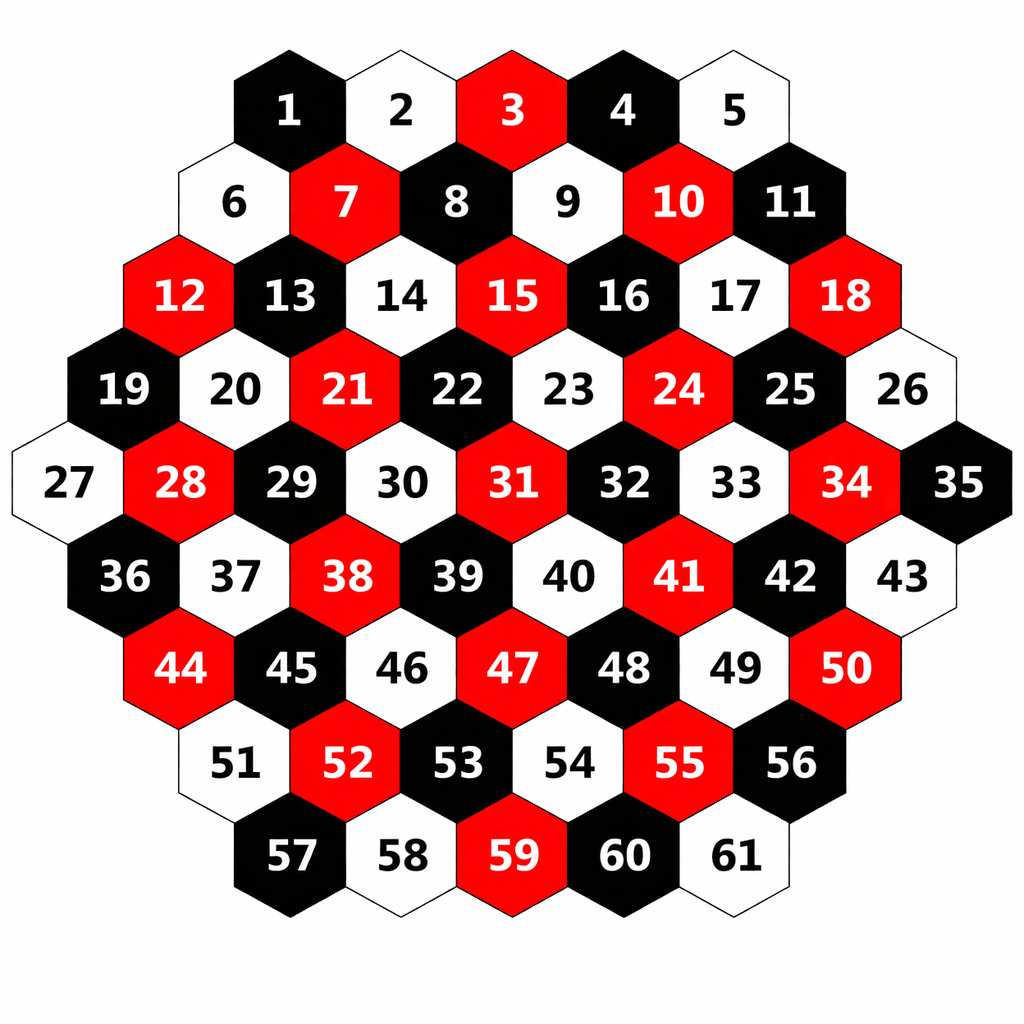
\includegraphics[scale=0.2]{implementation_of_the_game_model/images/numbered_tricolor_board.png}
    \caption{Board with numbered tiles from 1 to 61}
    \label{fig:numbered_tricolor_board}
\end{figure}

With these 3 insights we can conclude that a good data structure for the board state is an array of length 61 (for the number of tiles of the board) where each element is a 16 bits number. This is because, for each tile, we need to maintain the number of white and black pieces (from 0 to 18 for each color, which means we need 5 bits for each color, so 10 bits in total), as well as the owner of the tile (there are only 2 players, so we only need 1 bit; notice that for the neutral tiles, i.e. the empty tiles, it's possible to deduce the owner of the tile by the fact that there are no pieces at all, so no need for a "third" owner). A visual representation of the bit masking of each tile can be seen in Figure~\ref{fig:board_state_opti}. Finally, the player who has to move in the current position is maintained using a boolean value (0 = white has to move and 1 = black has to move).

\begin{figure}[h]
    \centering
    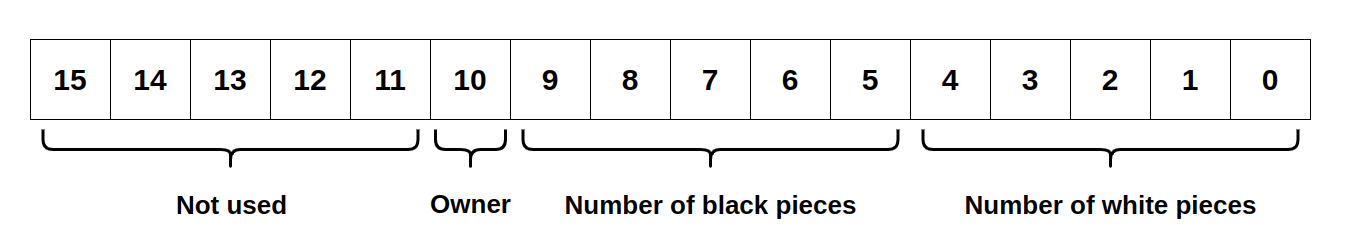
\includegraphics[scale=0.3]{implementation_of_the_game_model/images/board_state_opti.png}
    \caption{16-bit integer visual representation masking the state of a board}
    \label{fig:board_state_opti}
\end{figure}

This final compact structure of a board state has only a size of:
\begin{equation}
61 * 16 \text{ bits} + 8 \text{ bits} = 61 * 2 \text{ bytes} + 1 \text{ byte} = 123 \text{ bytes}
\label{eq:board_state_size}
\end{equation}
, which is really small. Therefore, making a copy of such a state is very fast.

Note: the different operations (getting the number of white pieces, black pieces, owner of a tile etc.) are done only using bitwise operations, making the implementation even faster than a naive one.

\subsection{Actions}

In any game, actions are the bridge between the different board states. In any position, the player that has to make the next move needs a set of actions to choose from (e.g. Player 1 decides to move 3 pieces of this stack to 2 tiles to the left like in Figure~\ref{fig:action_example}). When talking about performance, a model has to:

\begin{enumerate}
    \item generate all the possible actions for a board state as fast as possible
    \item use the least memory possible for the \textbf{action} structure
\end{enumerate}

\begin{figure}[h]
    \centering
    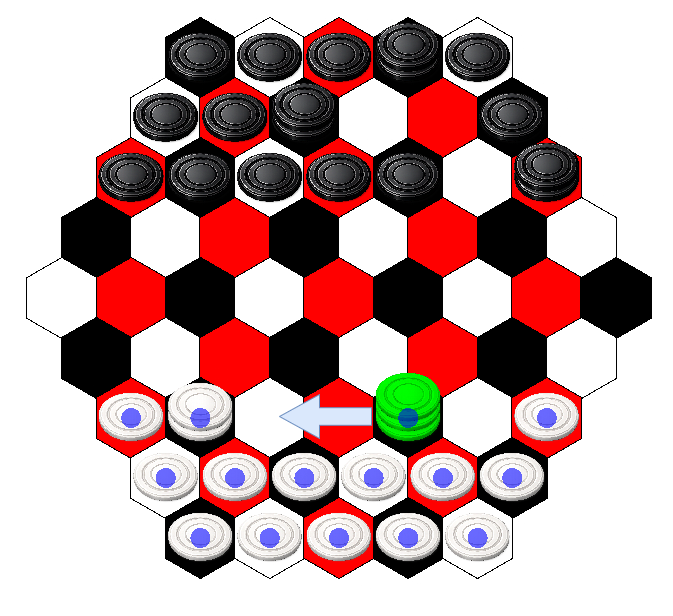
\includegraphics[scale=0.4]{implementation_of_the_game_model/images/action_example.png}
    \caption{Example of the action of Player 1 moving 3 pieces from a stack to 2 tiles to the left}
    \label{fig:action_example}
\end{figure}

Generating all the possible actions for a board state is a straightforward task. It only requires to iterate over all the owned board tiles by the player who's turn is and, depending on the number of pieces on the stack and the surrounding pieces in the 6 directions of the tile, check what actions are possible following the rules of the game described in a previous chapter. There isn't any major optimization that can be brought to this implementation of the actions generation.

For the minimization of memory usage of the \textbf{action} structure, it is sufficient to have the insight that to perfectly describe an action it is only needed to know the \textbf{from} tile, the \textbf{to} tile and the number of pieces moved from the \textbf{from} tile to the \textbf{to} tile. The tiles are numbered from 0 to 60, so 8 bits are sufficient to represent the \textbf{from} and \textbf{to} tiles. A player can theoretically move at most 35 pieces at the same time, so 8 bits are also sufficient to represent the number of moved pieces.

Therefore, the minimal representation of an action has only a size of:
\begin{equation}
8 \text{ bits} + 8 \text{ bits} + 8 \text{ bits} = 1 \text{ byte} + 1 \text{ byte} + 1 \text{ byte} = 3 \text{ bytes}
\label{eq:action_size}
\end{equation}
, which is really small.

\subsection{Game}

Once the Board State and Action structures are implemented, including their useful methods, simulating a game is very simple.

A normal game starts in the position shown in Figure~\ref{fig:board_setup}, where Player 1 (White) has to make the first move. From this point, each player chooses an action on their turn until:
\begin{enumerate}
    \item one of the players has no actions left, resulting in a win for the other player
    \item none of the players captured at least one enemy piece in the last 100 turns, resulting in a draw.
\end{enumerate}

\section{Basic Agents and User Interface}

\subsection{Random Agent}

The most basic and easy to implement "AI" agent is the Random Agent. As its name suggests, the Random Agent chooses every time a random action. It's useful to play and to explore the game using such an agent because:
\begin{itemize}
    \item it is used to analyze the different metrics of the game (e.g. duration,  branching factor etc.).
    \item it is used to test how good other AI agents are. If an AI agent has a 50\% win rate against the Random Agent, it means  it's very bad. However, if the AI agent wins 100\% of the games, it means it's already decent. 
    \item it already creates an opponent who is easy to play against, which gives humans the opportunity to learn basic game strategies.
\end{itemize}

\subsection{Human Agent and User Interface}

The Human Agent is also a basic agent because the action chosen at every turn is the one decided by a human.

To allow human players to compete against other humans or AI agents, a user interface was developed in C++ using the SFML library~\cite{sfml}. SFML is a high-level graphics library that simplifies the implementation of simple 2D games such as Tricolor.

When launching the game, it is needed to specify the two types of agents that will play against each other. The first one is Player 1 (White) and the second one is Player 2 (Black). Then, a window will pop on the screen (see Figure~\ref{fig:game_window}) and the game starts.

\begin{figure}[h]
    \centering
    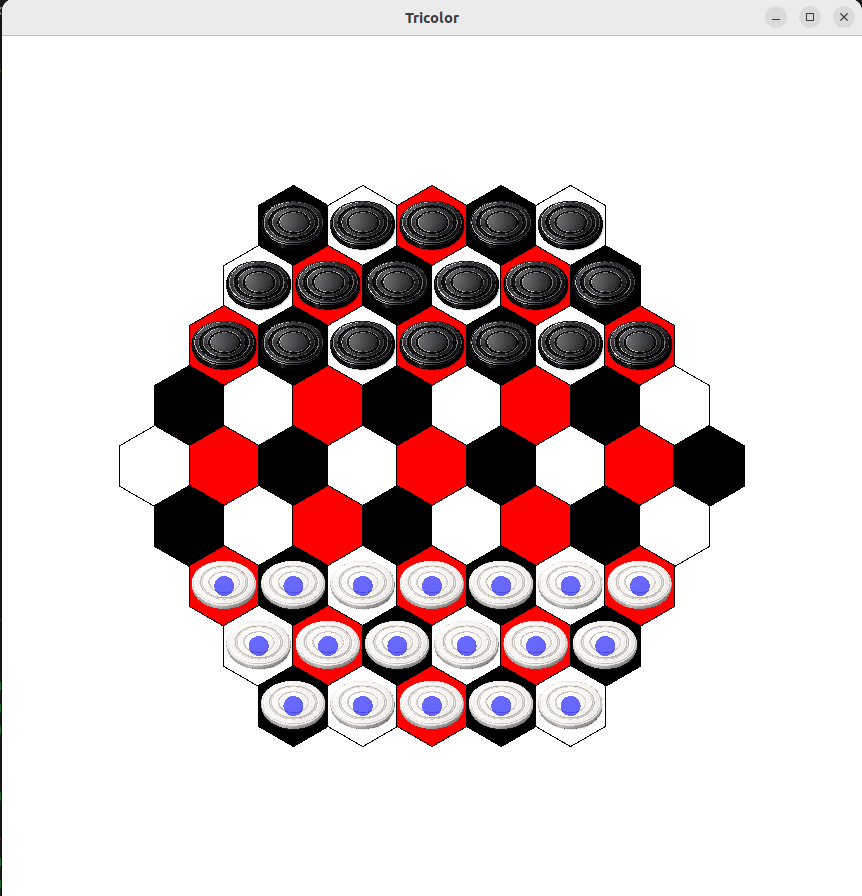
\includegraphics[scale=0.3]{implementation_of_the_game_model/images/game_window.png}
    \caption{Window showing the beginning of a game of Tricolor}
    \label{fig:game_window}
\end{figure}